\documentclass{standalone}
\usepackage{pgfplots}
\pgfplotsset{compat=1.18}
\usepgfplotslibrary{fillbetween}

\begin{document}

\definecolor{tab_blue}{HTML}{1F77B4}
\definecolor{tab_orange}{HTML}{FF7F0E}
\definecolor{tab_green}{HTML}{2CA02C}
\definecolor{tab_red}{HTML}{D62728}


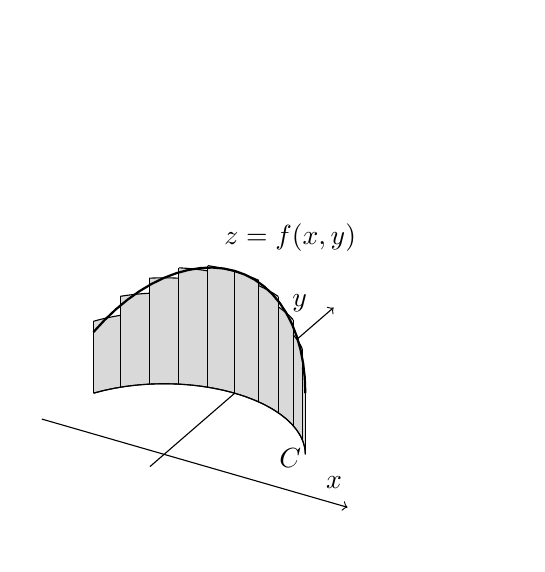
\begin{tikzpicture}[baseline]
\begin{axis}[
axis lines = middle,
unit vector ratio*=1 1 1,
scale=1.5, xmin=-1.0, xmax=1.5, ymin=-0.2, ymax=2.4, zmin = -0.2, zmax = 2.0,
hide z axis,
%grid = major,
view={30}{30},
ticks=none,
%xtick={0,1},
%ytick={0,1},
%ztick={0,1},
%xticklabels = {0,1},
%yticklabels = {0,1},
%zticklabels = {0,1},
xlabel=$x$,
ylabel=$y$,
%zlabel=$z$,
axis line style = {->},
]
% \fill[gray!20](axis cs:0.866,0.5,0) --(axis cs:0.866,0.5,0.5971) --  (axis cs:0.7274,0.6862,0.59712) -- (axis cs:0.7274,0.6862,0) -- cycle;
% \fill[gray!20](axis cs:0.7274,0.6862,0) -- (axis cs:0.7274,0.6862,0.7660) -- (axis cs:0.5495,0.8355,0.7660) -- (axis cs:0.5495,0.8355,0) -- cycle;
% \fill[gray!20](axis cs:0.5495,0.8355,0) -- (axis cs:0.5495,0.8355,0.8936) -- (axis cs:0.3420,0.9397,0.8936) -- (axis cs:0.3420,0.9397,0) -- cycle;
% \fill[gray!20](axis cs:0.3420,0.9397,0) -- (axis cs:0.3420,0.9397,0.9730) -- (axis cs:0.1161,0.9932,0.9730) -- (axis cs:0.1161,0.9932,0) -- cycle;
% \fill[gray!20](axis cs:0.1161,0.9932,0) -- (axis cs:0.1161,0.9932,1) -- (axis cs:-0.1161,0.9932,1) -- (axis cs:-0.1161,0.9932,0) -- cycle;
% \fill[gray!20](axis cs:-0.1161,0.9932,0) -- (axis cs:-0.1161,0.9932,0.9730) -- (axis cs:-0.3420,0.9397,0.9730) --(axis cs:-0.3420,0.9397,0) -- cycle;
% \fill[gray!20](axis cs:-0.3420,0.9397,0) -- (axis cs:-0.3420,0.9397,0.8936) -- (axis cs:-0.5495,0.8355,0.8936) --(axis cs:-0.5495,0.8355,0) -- cycle;
% \fill[gray!20](axis cs:-0.5495,0.8355,0) -- (axis cs:-0.5495,0.8355,0.7660) -- (axis cs:-0.7274,0.6862,0.7660) --(axis cs:-0.7274,0.6862,0) -- cycle;
% \fill[gray!20](axis cs:-0.7274,0.6862,0) --(axis cs:-0.7274,0.6862,0.5971)-- (axis cs:-0.866,0.5,0.5971) --(axis cs:-0.866,0.5,0) -- cycle;
%\addplot3[samples y=0,domain=5/6*pi:pi/6,postaction={decorate,decoration={markings,mark=between positions 0.2 and 0.8 step 0.2 with {\arrow[scale=1.4,>=stealth]{>};}}}]({cos(deg(x))},{sin(deg(x))},{0});
% \addplot3[samples y=0, domain=5/6*pi:pi/6] ({cos(deg(x))}, {sin(deg(x))}, 0);
% \addplot3[thick, samples y=0, domain=5/6*pi:pi/6] ({cos(deg(x))}, {sin(deg(x))}, {sin(deg(x))});

\pgfmathsetmacro{\a}{1/6*pi}
\pgfmathsetmacro{\b}{5/6*pi}
\addplot3[samples y=0, domain=\a:\b] ({cos(deg(x))}, {sin(deg(x))}, 0);
\addplot3[thick, samples y=0, domain=\a:\b] ({cos(deg(x))}, {sin(deg(x))}, {sin(deg(x))});
\pgfmathtruncatemacro{\Nsub}{10} 
\pgfmathsetmacro{\h}{(\b-\a)/\Nsub}

\pgfplotsforeachungrouped \i in {0,...,\Nsub-1}{
    \pgfmathsetmacro{\xleft}{\a+\i*\h}
    \pgfmathsetmacro{\xright}{\a+(\i+1)*\h} 
    \pgfmathsetmacro{\xmid}{\a+(\i+0.5)*\h}
    \pgfmathsetmacro{\height}{sin(deg(\xmid))} 
    \edef\doplot{\noexpand 
        \addplot3[domain=\xleft:\xright, samples y=0, name path=up] ({cos(deg(x))}, {sin(deg(x))}, {sin(deg(\xmid))});
    }
    \doplot
    \edef\doplot{\noexpand 
        \addplot3[domain=\xleft:\xright, samples y=0, name path=down] ({cos(deg(x))}, {sin(deg(x))}, 0);
    }
    \doplot
    \edef\doplot{\noexpand 
        \addplot3[fill=gray!30] fill between [of=up and down]; 
    }
    \doplot
    \edef\doplot{\noexpand 
        \addplot3[domain=0:\height, samples y=0] ({cos(deg(\xleft))}, {sin(deg(\xleft))}, {x});
    }
    \doplot
    \edef\doplot{\noexpand 
        \addplot3[domain=0:\height, samples y=0] ({cos(deg(\xright))}, {sin(deg(\xright))}, {x});
    }
    \doplot
}

\node at(axis cs:0.8,0.4,0){$C$};
\node at(axis cs:0.8,0.4,1.8){$z=f(x,y)$};
% \node at(axis cs:{cos(deg(\a+7*\h))}, {sin(deg(\a+7*\h))}, 0){$\bullet$};
% \node at(axis cs:{cos(deg(\a+6*\h))}, {sin(deg(\a+6*\h))}, 0){$\bullet$};
% \node at(axis cs:-0.55,0.8,0.15){$t_{k}$};
% \node at(axis cs:-0.35,0.9,0.15){$t_{k+1}$};
% \node at(axis cs:-0.4,0.75,0){$\Delta s_k$};
\end{axis}
\end{tikzpicture}

% \begin{tikzpicture}[baseline]
% \begin{axis}[
% axis lines = middle,
% unit vector ratio=1 1 1, 
% % axis equal=false,
% scale=1.2, 
% xmin=-2.1, xmax=2.1, ymin=-1.6, ymax=2.1, zmin = -0.2, zmax=2.1, 
% % grid = major,
% xtick={0},
% ytick={0},
% ztick={0}, 
% xticklabels = {},
% yticklabels = {},
% zticklabels = {},
% xlabel=$x$,
% ylabel=$y$,
% zlabel=$z$, 
% xlabel style={below right},
% ylabel style={above left},
% axis line style = {->},
% declare function={
%     myfunc(\x) = 0.5+0.8*(\x)^2;
% }
% ]
% \pgfmathsetmacro{\a}{-1.0}
% \pgfmathsetmacro{\b}{1.0}
% \addplot3[domain=-1:1, samples=100, samples y=0, thick] ({tan(deg(x))}, {x}, {myfunc(x)});
% \addplot3[domain=-1:1, samples=100, samples y=0, dashed] ({tan(deg(x))}, {x}, 0);
% \pgfmathtruncatemacro{\Nsub}{25} 
% \pgfmathsetmacro{\h}{(\b-\a)/\Nsub}

% \pgfplotsforeachungrouped \i in {0,...,\Nsub-1}{
%     \pgfmathsetmacro{\xleft}{\a+\i*\h}
%     \pgfmathsetmacro{\xright}{\a+(\i+1)*\h} 
%     \pgfmathsetmacro{\xmid}{\a+(\i+0.5)*\h}
%     \pgfmathsetmacro{\height}{myfunc(\xmid)} 
%     \edef\doplot{\noexpand 
%         \addplot3[domain=\xleft:\xright, samples y=0, name path=up] ({tan(deg(x))}, {x}, {\height});
%     }
%     \doplot
%     \edef\doplot{\noexpand 
%         \addplot3[domain=\xleft:\xright, samples y=0, name path=down] ({tan(deg(x))}, {x}, 0);
%     }
%     \doplot
%     \edef\doplot{\noexpand 
%         \addplot3[fill=gray!30] fill between [of=up and down]; 
%     }
%     \doplot
%     \edef\doplot{\noexpand 
%         \addplot3[domain=0:\height, samples y=0] ({tan(deg(\xleft))}, {\xleft}, {x});
%     }
%     \doplot
%     \edef\doplot{\noexpand 
%         \addplot3[domain=0:\height, samples y=0] ({tan(deg(\xright))}, {\xright}, {x});
%     }
%     \doplot
% }

% \end{axis}
% \end{tikzpicture}
\hspace{-15mm}

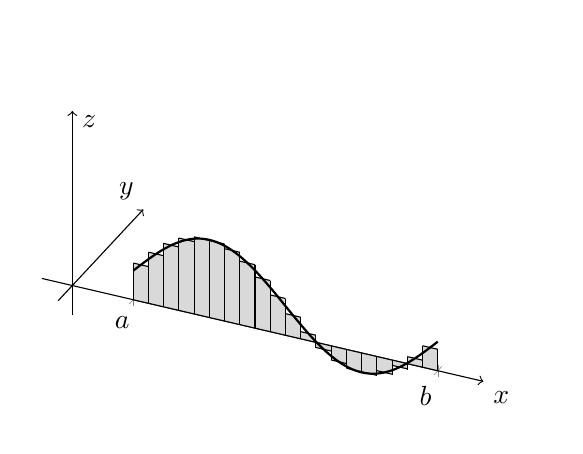
\begin{tikzpicture}[baseline]
\begin{axis}[
axis lines = middle,
unit vector ratio=1 1 1, 
% axis equal=false,
scale=1.2, 
xmin=-0.1, xmax=1.35, ymin=-0.1, ymax=0.5, zmin = -0.1, zmax=0.6, 
% grid = major,
xtick={0.2,1.2},
ytick={0},
ztick={0}, 
xticklabels = {$a$, $b$},
yticklabels = {},
zticklabels = {},
xlabel=$x$,
ylabel=$y$,
zlabel=$z$, 
xlabel style={below right},
ylabel style={above left},
axis line style = {->},
declare function={
    myfunc(\x,\a) = (sin(deg(2*pi*(\x-\a)))+0.6)/6;
}
]

\pgfmathsetmacro{\a}{0.2} 
\pgfmathsetmacro{\b}{1.2}
\pgfmathtruncatemacro{\Nsub}{20} 
\pgfmathsetmacro{\h}{(\b-\a)/\Nsub}

\pgfplotsforeachungrouped \i in {0,...,\Nsub-1}{
    \pgfmathsetmacro{\xleft}{\a+\i*\h}
    \pgfmathsetmacro{\xright}{\a+(\i+1)*\h} 
    \pgfmathsetmacro{\xmid}{\a+(\i+0.5)*\h}
    \pgfmathsetmacro{\height}{myfunc(\xmid,\a)} 
    \edef\doplot{\noexpand 
        \addplot3[domain=\xleft:\xright, samples y=0, name path=up] ({x}, 0, {\height});
    }
    \doplot
    \edef\doplot{\noexpand 
        \addplot3[domain=\xleft:\xright, samples y=0, name path=down] ({x}, 0, 0);
    }
    \doplot
    \edef\doplot{\noexpand 
        \addplot3[fill=gray!30] fill between [of=up and down]; 
    }
    \doplot
    \edef\doplot{\noexpand 
        \addplot3[domain=0:\height, samples y=0] ({\xleft}, 0, {x});
    }
    \doplot
    \edef\doplot{\noexpand 
        \addplot3[domain=0:\height, samples y=0] ({\xright}, 0, {x});
    }
    \doplot
}

\addplot3 [style=thick, domain=0.2:1.2, samples=100, samples y=0] ({x}, 0, {(sin(deg(2*pi*(x-0.2)))+0.6)/6});

\end{axis}
\end{tikzpicture}

\end{document}